%% -*- coding: utf-8 -*-
\documentclass[12pt,a4paper]{scrartcl} 
\usepackage[utf8]{inputenc}
\usepackage[english,russian]{babel}
\usepackage{indentfirst}
\usepackage{misccorr}
\usepackage{graphicx}
\usepackage{amsmath}
\begin{document}
\section{Введение}
\label{sec:intro}

% Что должно быть во введении
 Текстовая формулировка задачи: решение системы линейных алгебраических уравнений методом Крамера (количество неизвестных меньше 4).

 Теория: метод Крамера— способ решения систем линейных алгебраических уравнений с числом уравнений равным числу неизвестных с ненулевым главным определителем матрицы коэффициентов системы (причём для таких уравнений решение существует и единственно).
Для системы n линейных уравнений с n неизвестными

\label{sec:equation}
\begin{equation}
	\centering
	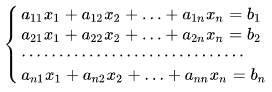
\includegraphics[width=0.4\textwidth]{f1.png}
	\label{eq:solv}
\end{equation}

с определителем матрицы системы Δ, отличным от нуля, решение записывается в виде

\label{sec:equation}
\begin{equation}
	\centering
	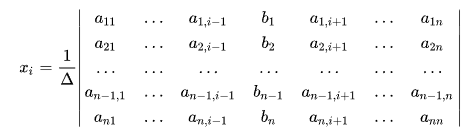
\includegraphics[width=0.4\textwidth]{f2.png}
	\label{eq:solv}
\end{equation}

(i-ый столбец матрицы системы заменяется столбцом свободных членов).
 
 Для решения использован Python 3

Пример приведен в пункте ~\ref{sec:exp} на стр.~\pageref{sec:example}.

\section{Ход работы}
\label{sec:exp}

\subsection{Код приложения}
\label{sec:exp:code}
\begin{verbatim}
# import numpy as np

class LinSys:

    _n = None
    _A = None
    _X = None
    _B = None

    _isFilled = False
    _isSolved = False

    def __init__(self, numberOfUnknowns: int) -> None:
        self._n = numberOfUnknowns
        # self._A = np.zeros((numberOfUnknowns, numberOfUnknowns))
        # self._X = np.zeros(numberOfUnknowns)
        # self._B = np.zeros(numberOfUnknowns)
        self._A = [[0] * numberOfUnknowns for i in range(0, numberOfUnknowns)]
        self._X = [0] * numberOfUnknowns
        self._B = [0] * numberOfUnknowns
        # 

    def processUserInput(self) -> None:
        print()
        print("Общий вид системы линейных уравнений:")
        print("  a11 * x1 + a12 * x2 + ... + a1n * xn = b1")
        print("  a21 * x1 + a22 * x2 + ... + a2n * xn = b2")
        print("  ...")
        print("  am1 * x1 + am2 * x2 + ... + amn * xn = bm")
        print("где")
        print("  m - количество уравнений")
        print("  n - количество переменных")
        print("  x1,x2,...,xn - неизвестные, которые надо определить")
        print("  a11,a12,...,amn - коэффициенты. Предполагаются известными")
        print("  b1,b2,...,bm - свободные члены. Предполагаются известными")
        print()
        print("В данном случае для решения используется метод Крамера. Потому количество уравнений m и количество неизвестных n должно совпадать (m = n)")
        print()

        for i in range(0, self._n):
            print("Введите коэффициенты уравнения", str(i + 1))
            for j in range(0, self._n):
                while True:
                    try:
                        self._A[i][j] = float(input(" a" + str(i + 1) + str(j + 1) + ": "))
                    except ValueError:
                        print("Введённое значение должно быть вещественным числом!")
                        continue
                    break

        print("Введите свободные члены уравнения")
        for i in range(0, self._n):
            while True:
                try:
                    self._B[i] = float(input(" b" + str(i + 1) + ": "))
                except ValueError:
                    print("Введённое значение должно быть вещественным числом!")
                    continue
                break
        
        self._isFilled = True
    
    def solve(self) -> bool:
        if not self._isFilled:
            print("Не все данные указаны. Систему решить невозможно")
            return False
        
        # det = np.linalg.det(self._A)
        det = self.det(self._A)
        # 
        if det == 0:
            print("Определитель матрицы коэффициентов равен нулю. Методом Крамера решить систему невозможно")
            return False

        # tmp = np.copy(self._A)
        tmp = [[0] * self._n for i in range(0, self._n)]
        for i in range(0, self._n):
            for j in range(0, self._n):
                tmp[i][j] = self._A[i][j]
        # 

        for k in range(0, self._n):
            for i in range(0, self._n):
                tmp[i][k] = self._B[i]
            
            # self._X[k] = np.linalg.det(tmp) / det
            self._X[k] = self.det(tmp) / det
            # 
            
            for i in range(0, self._n):
                tmp[i][k] = self._A[i][k]
        
        self._isSolved = True

        return True
    
    def printAnswer(self) -> None:
        if not self._isSolved:
            print("Внимание! Невозможно вывести решение: система ещё не решена. Попытка решения...")
            if self.solve():
                self.printAnswer()
            else:
                print("Неудача. Решить систему не получилось")
            return False
        
        print("Решения системы:")
        for i in range(0, self._n):
            print("x" + str(i + 1) + ":", round(self._X[i], 14))
    
    def det(self, mtx) -> int:
        if self._n == 1:
            return mtx[0][0]
        elif self._n == 2:
            return mtx[0][0] * mtx[1][1] - mtx[0][1] * mtx[1][0]
        elif self._n == 3:
            return mtx[0][0] * mtx[1][1] * mtx[2][2] - mtx[0][0] * mtx[1][2] * mtx[2][1] - mtx[0][1] * mtx[1][0] * mtx[2][2] + mtx[0][1] * mtx[1][2] * mtx[2][0] + mtx[0][2] * mtx[1][0] * mtx[2][1] - mtx[0][2] * mtx[1][1] * mtx[2][0]
        else:
            print("Вы пытаетесь найти определитель матрицы размером больше 3x3, что не предусмотрено условиями задания")
            exit()

class App:
    
    def __init__(self) -> None:
        pass

    def run(self) -> None:
        numberOfUnknowns = self.getInputNumberOfUnknowns()

        linsys = LinSys(numberOfUnknowns)

        linsys.processUserInput()

        if linsys.solve():
            linsys.printAnswer()
    
    def getInputNumberOfUnknowns(self) -> int:
        while True:
            try:
                numberOfUnknowns = int(input("Введите количество неизвестных (менее 4): "))
            except ValueError:
                print("Введённое значение должно быть целым числом!")
                continue
            if numberOfUnknowns < 1:
                print("Введённое значение не может быть меньше единицы!")
                continue
            elif numberOfUnknowns > 3:
                print("Введённое значение не может быть больше трёх!")
                continue
            return numberOfUnknowns

if __name__ == "__main__":
    app = App()
    app.run()
\end{verbatim}

\subsection{Пример работы}
\label{sec:example}
Пример работы представлен на рис.~\ref{fig:wex}
\begin{figure}[h]
	\centering
	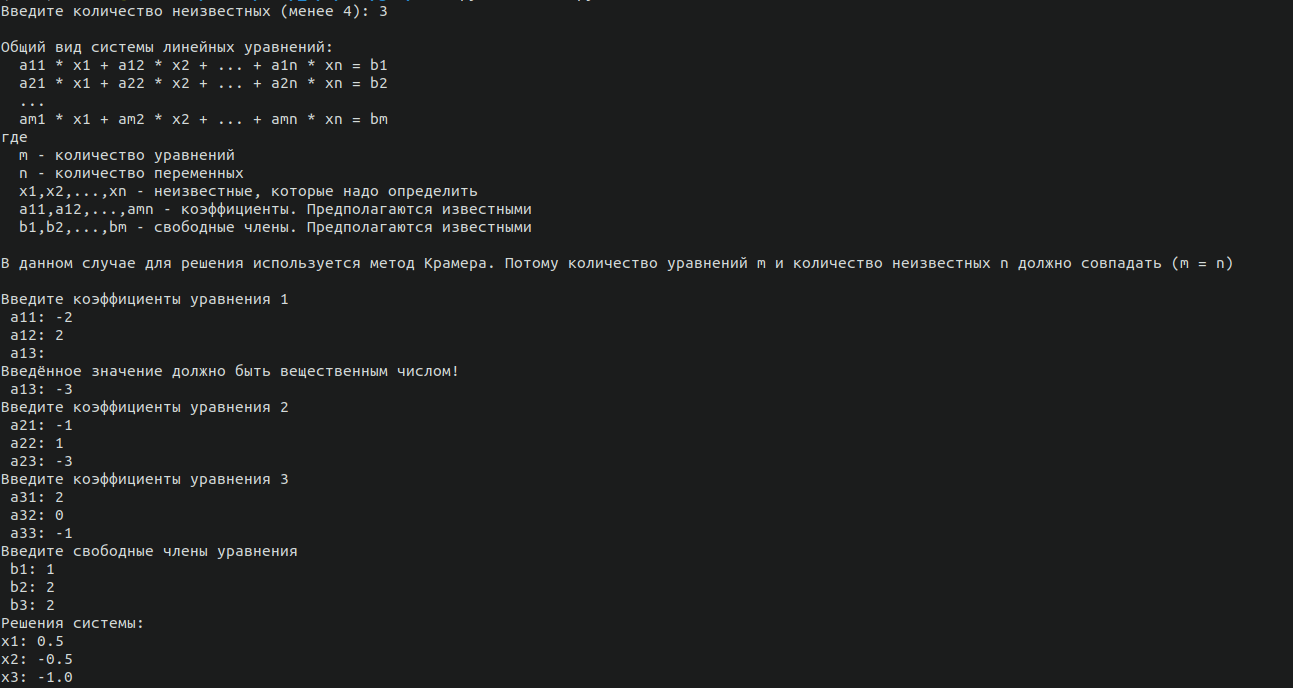
\includegraphics[width=1\textwidth]{example.png}
	\caption{Пример работы}\label{fig:wex}
\end{figure}

\end{document}